\section{Einleitung}
\label{sec:einleitung}
Als allgegenwärtige Anwendung von physikalischem Know-How ist die
Mikrowellentechnik kaum noch aus dem Alltag wegzudenken.
Von dem Haushaltsgerät Mikrowelle, das in wahrscheinlich jeder Küche der
westlichen Hemisphäre zu finden ist, bis zu Alarmanlagen wird diese Technik
in äußerst breit gefächerten Gebieten genutzt.
Ursprünglich schon zu Ende des zweiten Weltkrieges, als Frühwarnradar
entwickelt, wird Mikrowellenstrahlung schon einige Jahrzehnte eingesetzt.
Aus diesem Grund stellt sich die Untersuchung von Mikrowellen als interessante
Aufgabe für jeden Physiker dar.
Im Folgenden sollen verschiedene Welleneigenschaften mit Hilfe eines
Reflexklystrons untersucht und das Verhalten von Mikrowellen auf Hohlleitern
betrachtet werden.

\section{Grundlagen}
\label{sec:grundlagen}
\begin{wrapfigure}{r}{0.33\linewidth}
    \centering
    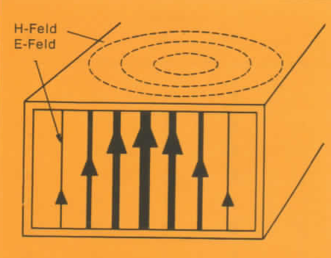
\includegraphics[width=0.9\linewidth]{img/hohlleiter.png}
    \caption{
        Der eransversal-elektrische $\text{TE}_{1,0}$-Modus in einem
        Rechteckhohlleiter, wie er in diesem Versuch untersucht wird
        \cite{V53}.
    }
    \label{fig:leiter}
\end{wrapfigure}
Als Mikrowellen wird elektromagnetische Strahlung im Frequenzbereich
von etwa \SI{300}{\mega \hertz} bis etwa \SI{300}{\giga \hertz} bezeichnet.
Niedrigere Frequenzen gehen über in Funkwellen während noch höhere Frequenzen
in den Bereich des infraroten Lichts reichen.

Elektromagnetische Wellen breiten sich im Vakuum kugelförmig aus, wobei ihre
Intensität mit $1 / r^2$ abnimmt.
Jede elektromagnetische Welle kann jedoch auch in verschiedenen metallischen
Wellenleitern transportiert werden, wobei -- je nach Leiter -- theoretisch
keine Verluste auftreten.
Der hier untersuchte Hohlleiter weist einen rechteckigen Querschnitt auf,
wie in Abbildung \ref{fig:leiter} dargestellt.
Leiter diese Art werden für Mikrowellen häufig verwendet.

\subsection{Moden}
\label{subse:moden}
Wie in einem Einfachen Hohlraumresonator können Wellen in einem Hohlleiter
konstruktiv oder destruktiv interferieren.
Ähnlich zu einer stehenden Welle in jenem Resonator kann sich dabei eine Welle
mit Bäuchen und Knoten zwischen den Leiterwänden ausbilden, die eine gewisse
Ausbreitungskomponente entlang der Leiterachse besitzt.
Für die Wellenlänge $\lambda$ der Mikrowellen muss dabei die Beziehung
\begin{equation*}
    \lambda \overset{!}{>} \lambda_\text{c} = 2a\,,
\end{equation*}
gelten, wobei $a$ den Abstand der Hohlleiterwänder bezeichnet und
$\lambda_\text{c}$ die Wellenlänge darstellt, unterhalb derer der Hohlleiter
keine Energie mehr transportiert -- die sogenannte Cut-Off-Wellenlänge.

Die fortlaufenden Wellen bilden unter dieser Voraussetzung verschiedene Moden,
die anhand der Ausprägung des elektrischen oder magnetischen Feldanteils
bezeichnet werden.
Bei transversal-elektrischen (TE-) Moden schwingt das elektrische Feld
senkrecht zur Ausbreitungsrichtung, während dies das magnetische Feld
bei transversal-magnetischen (TM-) Moden macht.
Die Anzahl der Schwingungsbäuche senkrecht zur Ausbreitungsrichtung $z$
entspricht dabei der Modenzahl $n$, $m$ in $x$- beziehungsweise $y$-Richtung
(siehe Abbildung \ref{fig:leiter}).

\subsection{Erzeugung von Mikrowellen mit einem Klystron}
\label{subsec:klystron}
Mikrowellen können mit Hilfe verschiedener Geräte erzeugt werden.
Das Klystron nutzt die von beschleunigten Elektronen abgegebene Strahlung.
Dafür werden die Elektronen resonant zwischen zwei Elektroden reflektiert
(Reflex-Klystron), wobei die abgegebene Bremsstrahlung im bereich der
Mikrowellen liegt.

Aus einer Kathode werden Elektronen emittiert und in Richtung eines positiv
geladenen Gitters beschleunigt.
Anschließend erreichen sie den Reflektor, bei dem sie auf Grund seiner
negativen Ladung abgebremst und in die entgegengesetzte Richtung beschleunigt
werden.
Wird nun eine periodische Spannung mit sich änderndem Vorzeichen zwischen
Reflektor und Gitter angelegt, beginnen die Elektronen zu schwingen und
passieren regelmäßig den Resonator.
Falls sie im Resonator abgebremst werden, geben sie Energie ab, die als
Mikrowellenstrahlung ausgekoppelt wird.
Dabei tritt eine periodische Abhängigkeit der Leistung
von der Verweildauer der Elektronen vor dem Reflektor auf, die durch die
Reflektorspannung $V$ beeinflusst werden kann.
Zudem kann der Abstand der Reflektorplatte mechanisch verändert werden,
was einen größeren Einfluss auf die Frequenz hat, in der das Klystron schwingt.
Insgesamt ergeben sich somit zwei Möglichkeiten zur Beeinflussung der
Ausgangsleistung und -frequenz, die elektronische und mechanische Abstimmung.
Abbildung \ref{fig:aufbau} stellt den schematischen Aufbau des Klystrons dar.
Abbildung \ref{fig:output} zeigt die Ausgangsleistung in Abhängigkeit der
Reflektorspannung.
\begin{figure}[p]
    \centering
    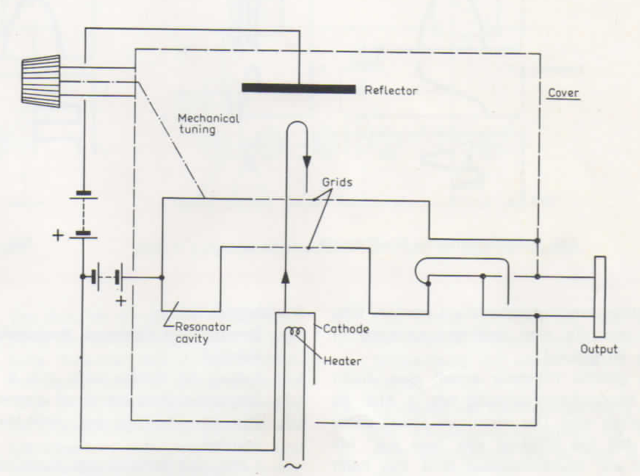
\includegraphics[width=0.9\linewidth]{img/aufbau.png}
    \caption{
        Schematische Darstellung des Aufbaus eines Reflex-Klystrons
        zur Erzeugung von Mikrowellenstrahlung \cite{V53}.
    }
    \label{fig:aufbau}
\end{figure}
\begin{figure}[p]
    \centering
    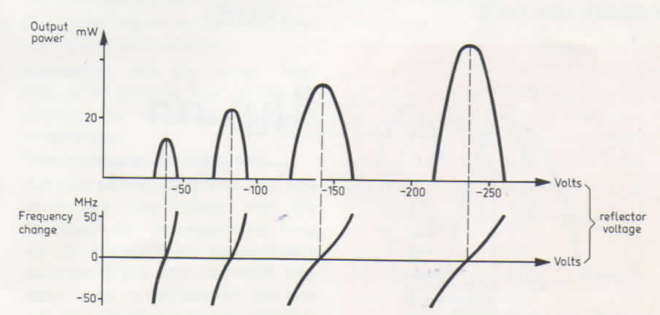
\includegraphics[width=0.9\linewidth]{img/output.png}
    \caption{
        Ausgangsleistung des Klystrons in Abhängigkeit zur Reflektorspannung
        \cite{V53}.
    }
    \label{fig:output}
\end{figure}
\clearpage

\section{Durchführung}
Im Folgenden wird das Klystron mit einer Rechteckspannung amplitudenmoduliert.
Die Rechteckspannung wird dafür auf den Reflektor gegeben und die abgegebene
Leistung zeitabhängig gemessen.
Die Leistung wird dabei mit einem Stehwellenmessgerät (SWR-Meter) gemessen.
Alternativ lassen sich mit Hilfe eines Oszillographen die Modenkurven, wie in
Abbildung \ref{fig:moden} dargestellen.
Dabei muss das Zeitsignal auf den $x$- und das Leistungssignal auf die
$y$-Achse des Oszillographen gelegt werden.
Der Versuchsaufbau ist Exemplarisch in Abbildung \ref{fig:aufbau_microwave.png}
dargestellt.
\begin{figure}[p]
    \centering
    \begin{subfigure}{0.6\linewidth}
        \centering
        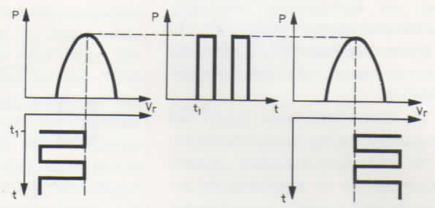
\includegraphics[width=0.8\linewidth]{img/moden.png}
        \caption{
            Rechteckmodulation des Klystrons
        }
        \label{fig:moden}
    \end{subfigure}
    \begin{subfigure}{0.39\linewidth}
        \centering
        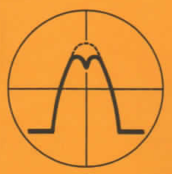
\includegraphics[width=0.8\linewidth]{img/dip.png}
        \caption{
            Dip in der Klystron-Leistung
        }
        \label{fig:dip}
    \end{subfigure}
    \caption{
        Modulationsschema des für eine Rechteckmodulation des Klystrons,
        sowie Rückgang der Klystron-Leistung, hervorgerufen durch einen
        Frequenzmesser, der auf eine Klystron-Mode eingestellt ist
        \cite{V53}.
    }
    \label{fig:moden-dip}
\end{figure}
\begin{figure}[p]
    \centering
    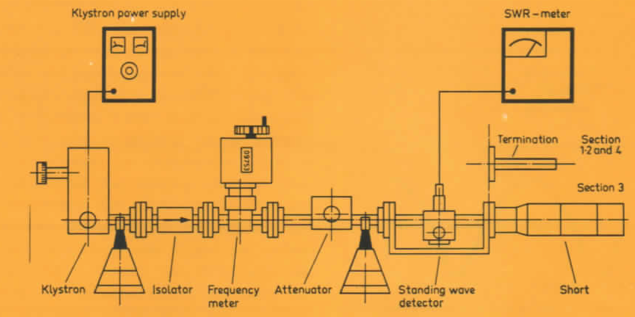
\includegraphics[width=0.8\linewidth]{img/aufbau_microwave.png}
    \caption{
        Schematische Abbildung des Versuchsaufbaus. Statt des
        SWR-Meters wird bei einigen Messungen ein Oszillograph angeschlossen
        und der Standing-Wave-Detector durch einen Detektor ersetzt.
    }
    \label{fig:aufbau_microwave}
\end{figure}
Die Mikrowellenfrequenz kann dabei mit einem Frequenzmesser überprüft werden.
Dieser wird durch einen variablen Resonator realisiert. Falls die
erzeugte Frequenz genau der Resonatorfrequenz entspricht, wird Welle zu einem
Teil absorbiert, was in einem messbaren Rückgang der Leistung (Dip)
resultiert und in Abbildung \ref{fig:dip} deutlich erkennbar ist.

\subsection{Messung verschiedener Aufbaueigenschaften}
\label{subsec:messung}
Wenn sich auf dem Oszillographen ein Dip erkennen lässt, kann mit dessen Hilfe
die Abstimmempfindlichkeit $A$ des Aufbaus berechnet werden.
Hierfür wird der Dip durch variation der Frequenz $f$ des Frequenzmessers auf
die halbe Höhe der Modenfigur beidseitig neben dem Modenmaximum verschoben.
Dabei wird die Reflektorspannung $V$ notiert.
Es gilt
\begin{equation}
    \label{eqn:empfindlichkeit}
    A = \frac{f^\prime - f^{\prime\prime}}{V^\prime - V^{\prime\prime}}\,.
\end{equation}
Die gestrichenen Größen sind dabei die Messwerte neben dem Modenmaximum.

Neben der Abstimmempfindlichkeit kann die Hohlleiterfrequenz statt durch
direkte Messung mit Erzeugung einer stehenden Welle bestimmt werden.
Dafür muss der Frequenzmesser verstimmt werden, um keine Leistung zu
absorbieren.
Es wird ein Kurzschluss mit variablem Detektor für stehende Wellen
angeschlossen.
Durch Variation der Detektorstellung lassen sich dann Leistungsminima finden,
die durch einen Knoten der stehenden Welle entstehen.
Die Wellenlänge $\lambda_\text{g}$ im Hohlleiter entspricht dann dem doppelten
Abstand benachbarter Minima. Mit der Lichtgeschwindigkeit $c$
und der Breite $a$ des Hohlleiters gilt für die Frequenz $f$ der stehenden
Welle
\begin{equation}
    \label{frequenz}
    f = c\cdot\sqrt{\left(\frac{1}{\lambda_\text{g}}\right)^2 + \left(\frac{1}{2a}\right)^2} \,.
\end{equation}

\clearpage
